\documentclass[border=0.125cm]{standalone}
\usepackage{tikz}
\usetikzlibrary{positioning}
\begin{document}

\tikzset{%
  every neuron/.style={
    circle,
    draw,
    minimum size=1cm
  },
  neuron missing/.style={
    draw=none, 
    scale=4,
    text height=0.333cm,
    execute at begin node=\color{black}$\vdots$
  },
}

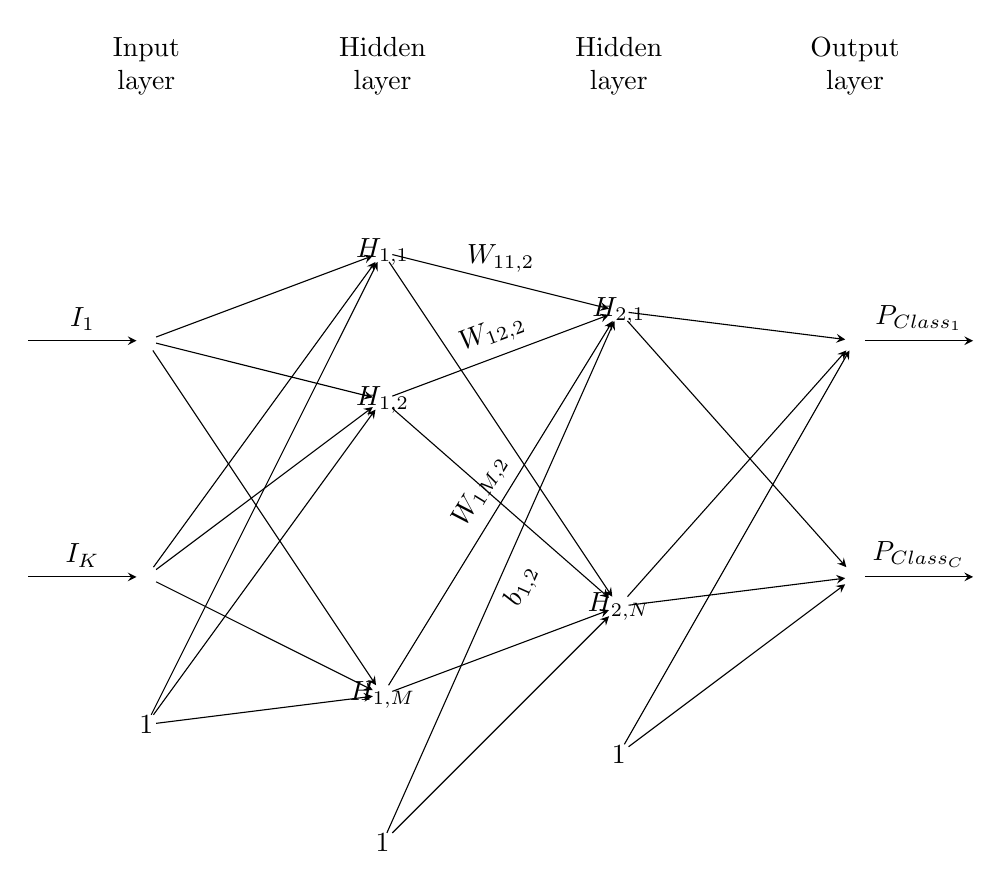
\begin{tikzpicture}[x=1.5cm, y=1.5cm, >=stealth]

\foreach \m/\l [count=\y] in {1,missing,2}
  \node [every neuron/.try, neuron \m/.try] (input-\m) at (0,1-\y) {};

\foreach \m/\l [count=\y] in {3}
\node [every neuron/.try, neuron \m/.try] (input-\m) at (0,-2-1*1.25) {};

\foreach \m [count=\y] in {1,2,missing,3,4}
  \node [every neuron/.try, neuron \m/.try ] (hidden1-\m) at (2,2-\y*1.25) {};

\foreach \m [count=\y] in {1,missing,2,3}
\node [every neuron/.try, neuron \m/.try ] (hidden2-\m) at (4,1.5-\y*1.25) {};

\foreach \m [count=\y] in {1,missing,2}
  \node [every neuron/.try, neuron \m/.try ] (output-\m) at (6,1-\y) {};

\foreach \l [count=\i] in {1,K}
  \draw [<-] (input-\i) -- ++(-1,0)
    node [above, midway] {$I_{\l}$};
    
\node [] at (input-3.center) {1};

\foreach \l [count=\i] in {1,2,M}
  \node [] at (hidden1-\i.center) {$H_{1,\l}$};
  \node [] at (hidden1-4.center) {1};

\foreach \l [count=\i] in {1,N}
	\node [] at (hidden2-\i.center) {$H_{2,\l}$};
	\node [] at (hidden2-3.center) {1};

%\foreach \l [count=\i] in {1,2,3}
  \draw [->] (output-1) -- ++(1,0)
    node [above, midway] {$P_{Class_1}$};
      \draw [->] (output-2) -- ++(1,0)
    node [above, midway] {$P_{Class_C}$};

\foreach \i in {1,...,2,3}
  \foreach \j in {1,...,3}
    \draw [->] (input-\i) -- (hidden1-\j);

\foreach \i in {1,...,3,4}
	\foreach \j in {2,...,2}
	\draw [->] (hidden1-\i) -- (hidden2-\j);
	\draw [->] (hidden1-4)--(hidden2-1)
		node [below,midway,sloped]{$b_{1,2}$};
	
\draw [->] (hidden1-1) -- (hidden2-1)
	node [above, midway] {$W_{11,2}$};

\draw [->] (hidden1-2) -- (hidden2-1)
node [above, midway, sloped] {$W_{12,2}$};

\draw [->] (hidden1-3) -- (hidden2-1)
node [above, midway,sloped] {$W_{1M,2}$};

\foreach \i in {1,...,2,3}
  \foreach \j in {1,...,2}
    \draw [->] (hidden2-\i) -- (output-\j);

\foreach \l [count=\x from 0] in {Input, Hidden,Hidden,Output}
  \node [align=center, above] at (\x*2,2) {\l \\ layer};

\end{tikzpicture}

\end{document}